\section{A tensor obstruction on a graph}\label{sec:tensors}

The obstruction needed here is governed by the plumbing graph associated
to a hypothetical marked filling.  We prove that formal data on the
corresponding cut pieces force an assignment of every edge to one endpoint
such that, at each vertex, no prescribed set of incident edges is assigned
entirely to that vertex.  On the colored odd cycle used in the construction,
no such assignment exists.  The truncated differential forms and the two
successive homologies in the proof come from the finite tensor obstruction of
\cite[Section~3]{MT}.  We give the algebraic argument in full, including the
passage from two vertices to an arbitrary graph.

\subsection{The incidence theorem}

Let \(\Gamma=(V,E)\) be a finite multigraph without loops.  Distinguish its
two endpoints as \(v_+(e)\) and \(v_-(e)\) for every \(e\in E\).  Write
\(E_+(v)\), \(E_-(v)\), and \(E(v)\) for the edges having plus endpoint
\(v\), minus endpoint \(v\), and either endpoint \(v\), respectively.
An endpoint assignment is a function \(a:E\to V\) with
\(a(e)\in\{v_+(e),v_-(e)\}\).

For a field \(K\), denote by \(K\langle h\rangle\) the ring of algebraic
power series, viewed as the henselization of \(K[h]_{(h)}\) inside
\(K[[h]]\).  Thus its elements have finite pointed \(\acute{e}\)tale
presentations.  All derivatives below act on internal coordinates; the
parameters \(t_e\) are held fixed.  Empty products are equal to one, and a
coordinate block is allowed to have dimension zero.

\begin{theorem}[Endpoint assignment]\label{ten:assignment}
Let \(K\) have characteristic zero, and let \(\Gamma\) be a finite
loopless multigraph with distinguished endpoints as above.  For each edge
\(e\), choose a coordinate block \(h_e\) of dimension \(N_e\geq0\) and
functions \(F_e,b_e\in K\langle h_e\rangle\).  For each vertex \(v\),
choose a family \(\mathcal L_v\) of nonempty subsets of \(E(v)\), and set
\begin{align}
 T_v&=K[t_e:e\in E_+(v)]/(t_e^2:e\in E_+(v)),\label{ten:parameters}\\
 \mathcal S_v(h,t)
 &=\sum_{e\in E_+(v)}(F_e(h_e)+t_e b_e(h_e))
       -\sum_{e\in E_-(v)}F_e(h_e).\label{ten:vertex-potential}
\end{align}
Suppose there are formal parametrizations
\[
 M_v(y_v,t)\in (y_v,t)T_v[[y_v]]^{\sum_{e\in E(v)}N_e},
 \qquad y_v=(y_{v,1},\ldots,y_{v,a_v}),
\]
satisfying the following conditions.
\begin{enumerate}
 \item The central tangent maps \(A_v=\partial_{y_v}M_v(0,0)\) are
 injective, and the difference map
 \begin{equation}\label{ten:transversality}
 \begin{split}
 \Lambda:\bigoplus_{v\in V}K^{a_v}&\longrightarrow
                         \bigoplus_{e\in E}K^{N_e},\\
 (\xi_v)_v&\longmapsto
 \bigl((A_{v_+(e)}\xi_{v_+(e)})_e
             -(A_{v_-(e)}\xi_{v_-(e)})_e\bigr)_e
 \end{split}
 \end{equation}
 is an isomorphism.
 \item One has \(\mathcal S_v(M_v(y_v,t),t)=0\) identically for every
 vertex \(v\).
 \item For every \(L\in\mathcal L_v\), put
 \(I=L\cap E_+(v)\) and \(J=L\cap E_-(v)\).  Then
 \begin{equation}\label{ten:law-membership}
 \left(\prod_{i\in I}t_i\right)
 \left(\prod_{j\in J}b_j\right)(M_v)
 \in
 \bigl((\partial_h\mathcal S_v)(M_v)\bigr)
                         \subset T_v[[y_v]].
 \end{equation}
 The ideal on the right is generated by all restricted internal
 partial derivatives of \(\mathcal S_v\).
\end{enumerate}
There is an endpoint assignment \(a:E\to V\) such that, for every
\(v\in V\) and \(L\in\mathcal L_v\), at least one edge of \(L\) is
assigned to its endpoint other than \(v\).
\end{theorem}

Injectivity in the first condition makes every parametrization a smooth
formal graph, also over the full parameter ring \(T_v\).  In particular,
nilpotent constant displacements are permitted.  The relations in
\eqref{ten:parameters} are individual relations: products of distinct
parameters remain present.

Before proving the theorem, we record its consequence for the graph used
in the chamber construction.

\begin{corollary}[Colored odd cycles]\label{ten:odd-cycle}
Let \(d\geq3\) be odd.  On the cycle with vertices \(\mathbb Z/d\mathbb Z\),
replace every neighboring pair by five red and five blue parallel
edges.  Distinguish the two endpoints of each edge arbitrarily.  At
each vertex let \(\mathcal L_v\) consist of every four-element subset
of incident edges containing two red and two blue edges.  There are
no data satisfying the hypotheses of Theorem~\ref{ten:assignment} for
this graph and these law families.
\end{corollary}

\begin{proof}
An assignment supplied by Theorem~\ref{ten:assignment} cannot assign
two red and two blue edges to the same vertex.  Hence every vertex
receives at most one edge in at least one of the two colors.
Call such a color deficient at that vertex.  Two adjacent vertices
cannot share a deficient color: each of the five edges of that color
joining them must be assigned to one of the two vertices, whereas together
the two vertices could receive at most two.  Thus the nonempty sets of
deficient colors at adjacent vertices are disjoint.  Each such set
is consequently a singleton, and the deficient colors alternate
around the cycle.  This is impossible when \(d\) is odd; see
Figure~\ref{ten:cycle-figure}.
\end{proof}

\begin{figure}[hbp]
\centering
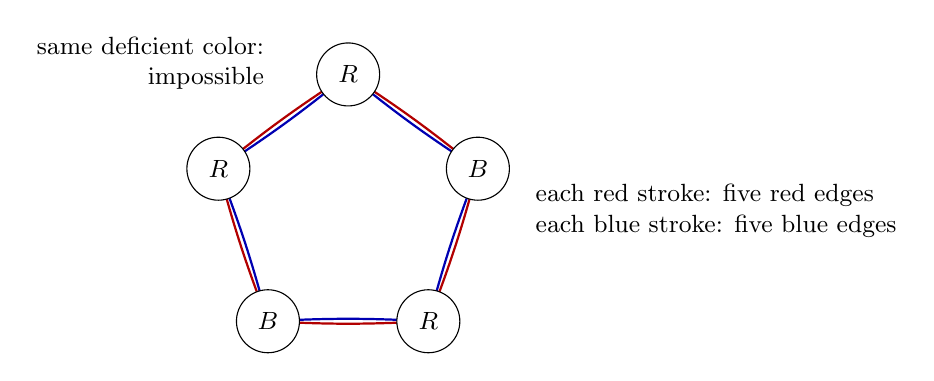
\begin{tikzpicture}[scale=1.05,
  deficiency/.style={circle,draw,fill=white,minimum size=8mm,inner sep=0pt},
  every node/.style={font=\small}]
 \coordinate (v0) at (90:1.65);
 \coordinate (v1) at (18:1.65);
 \coordinate (v2) at (-54:1.65);
 \coordinate (v3) at (-126:1.65);
 \coordinate (v4) at (162:1.65);
 \foreach \i/\j in {0/1,1/2,2/3,3/4,4/0}{
  \draw[red!70!black,line width=0.8pt]
    (v\i) to[bend left=3] (v\j);
  \draw[blue!70!black,line width=0.8pt]
    (v\i) to[bend right=3] (v\j);
 }
 \node[deficiency] at (v0) {\(R\)};
 \node[deficiency] at (v1) {\(B\)};
 \node[deficiency] at (v2) {\(R\)};
 \node[deficiency] at (v3) {\(B\)};
 \node[deficiency] at (v4) {\(R\)};
 \node[anchor=south east,align=right] at (-0.9,1.35)
    {same deficient color:\\impossible};
 \node[anchor=west,align=left] at (2.15,0)
    {each red stroke: five red edges\\
     each blue stroke: five blue edges};
\end{tikzpicture}
\caption{The deficient-color contradiction on a five-cycle.
Letters denote colors in which the vertex receives at most one edge.
Adjacent vertices must have different letters, so the forced alternation
fails when the cycle closes.}\label{ten:cycle-figure}
\end{figure}

For the application, a hypothetical filling is cut into vertex pieces
meeting along three-dimensional edge cuts.  Section~\ref{sec:formal}
constructs the functions \(F_e,b_e\) and graphs \(M_v\) from connection
data on these pieces.  The three hypotheses arise from transversality,
cancellation of boundary actions, and disk-bounding marked laws; the
gradient ideals encode flatness in the chosen formal families.

It remains to prove Theorem~\ref{ten:assignment}.  The proof converts
the vertex graphs into tensors whose contraction along
all edges is nonzero.  The law memberships force certain coefficients of
these tensors to vanish.  A nonzero term of the contraction then chooses
the required endpoint for every edge.  The argument uses the given graph
directly; it does not require a bipartition.

\subsection{Reduction to a finite-dimensional setting}

\begin{lemma}[Finite specialization]\label{ten:specialization}
If data satisfying the hypotheses of Theorem~\ref{ten:assignment} exist,
the same algebraic identities, ideal memberships, and tangent conditions
can be realized over a finite field of characteristic \(q\), for arbitrarily
large primes \(q\), with the same graph and law families.  The functions
\(F_e,b_e\) remain algebraic and depend only on their own edge block.
\end{lemma}

\begin{proof}
At each vertex choose a linear projection of the ambient coordinate space
onto \(K^{a_v}\) that is invertible on the central tangent image.
Its composite with \(M_v\) has a formal inverse over \(T_v\), with
parameters fixed.  The possible constant displacement lies in the
nilpotent ideal \((t)\), so the substitution is well defined.  Reparametrize
to make this projection of \(M_v\) equal to \(y_v\).

For a subset \(A\subset E_+(v)\), write \(t_A=\prod_{e\in A}t_e\).
Expand the graph and every coefficient witnessing
\eqref{ten:law-membership} in the finite basis \(\{t_A\}_A\) of \(T_v\).
All the resulting unknown coefficient series have the same independent
variables \(y_v\).  Represent the fixed edge functions on pointed
\(\acute{e}\)tale neighborhoods.  Implicit differentiation expresses their
ambient derivatives in the same finite presentations, with inverse
Jacobian determinants included among the units.  Auxiliary variables for
these presentations and units turn the following requirements into a
finite polynomial system in the unknown coefficient series:
the presentation equations, the fixed graph projection, the vanishing of
\(\mathcal S_v\), and all the ideal-membership identities.  No derivative
of an unknown coefficient series occurs.

Artin approximation over \(K[y_v]_{(y_v)}^h\)
\cite[Theorem~1.10]{Artin1969} gives algebraic coefficient series that
still solve this polynomial system exactly and agree with the original
solution through first order.  In particular, the central graph tangent
and all chosen branch centers are preserved.
Apply it separately at each vertex.  These systems share only the fixed
edge functions, and their mutual transversality is a condition on the
preserved first jets.  Thus no nested approximation is involved.  When
\(a_v=0\), the coefficient system already consists of equations over
\(K\), and no approximation is needed there.
The preserved branch centers and invertible Jacobians identify the
auxiliary solutions uniquely with the compositions of the fixed edge
germs and the approximated graph.

We now have finitely many algebraic germs and exact identities between
them.  Each is represented at a finite stage of a henselization, and every
identity holds at a sufficiently large finite stage.  Descend these
presentations, compositions, branch centers, and identities to a finitely
generated integral \(\mathbb Z\)-subalgebra \(A\subset K\).  Include the
inverse \(\acute{e}\)tale Jacobians and the inverse determinant in
\eqref{ten:transversality}.  The implicit differentiation identities
descend as well, so specialization preserves the meaning of the gradient
entries.  The original presentations for \(F_e,b_e\) still use only
\(h_e\).

There are specializations of \(A\) to finite fields in arbitrarily large
characteristic.  Indeed, a maximal quotient of the nonzero finite-type
\(\mathbb Q\)-algebra \(A\otimes\mathbb Q\) is a number field \(E_0\).
The images of a finite set of generators of \(A\), including all the
specified inverses, lie in \(\mathcal O_{E_0}[1/d_0]\) for some positive
integer \(d_0\).  Reduction at a prime above any rational prime not
dividing \(d_0\) gives the desired specialization.  All declared units
remain invertible.  The pointed \(\acute{e}\)tale presentations therefore
give formal germs satisfying the same identities and tangent conditions
over the residue field.
\end{proof}

Fix such a field \(k\) of characteristic \(q>2\).  For each edge define
\[
 R_e=k[h_{e,1},\ldots,h_{e,N_e}]/
                    (h_{e,1}^q,\ldots,h_{e,N_e}^q),
 \qquad
 \Omega_e=R_e\otimes_k
             \bigwedge\langle \mathrm dh_{e,1},\ldots,
                                      \mathrm dh_{e,N_e}\rangle .
\]
Let \(\mathrm d\) denote the exterior differential.  It is well defined
because \(\mathrm d(h_{e,r}^q)=0\).  We always use the graded tensor
convention: moving homogeneous factors of exterior degrees \(r,s\) past
one another contributes \((-1)^{rs}\).

Order the coordinates in each block and define integration to be zero
outside exterior degree \(N_e\), and otherwise to extract the coefficient
of \(\prod_r h_{e,r}^{q-1}\) from the coefficient of
\(\mathrm dh_{e,1}\wedge\cdots\wedge\mathrm dh_{e,N_e}\).
For a zero-dimensional block, this is the identity on \(k\).  Integration
kills exact forms, since differentiating a monomial cannot produce
exponent \(q-1\) in the differentiated coordinate.  Thus
\begin{equation}\label{ten:integration-parts}
 \int\mathrm d\alpha\wedge\beta
       =-(-1)^{|\alpha|}\int\alpha\wedge\mathrm d\beta
\end{equation}
for homogeneous forms.

These constructions extend to products of edge blocks and to the
square-free parameter rings by tensoring and differentiating only the
internal coordinates.  They turn the formal graphs into finite tensors
without discarding any of the parameter coefficients needed by the laws.

The projection normalization in Lemma~\ref{ten:specialization} also
provides explicit graph equations.  Complete its projected coordinates
\(x\) to linear ambient coordinates \((x,z)\).  The graph is then
\((x,f(x,t))\), and its equations are \(c_s=z_s-f_s(x,t)\).
We use these equations for the vertex graphs in the next construction.

\begin{lemma}[Graph forms]\label{ten:graph-forms}
Let \(c_1,\ldots,c_r\) be graph equations for a smooth formal graph over
one of the square-free parameter rings, centered modulo its parameter
ideal.  In the truncated differential forms of its ambient space, set
\begin{equation}\label{ten:graph-form}
 U_c=\bigwedge_{s=1}^r c_s^{q-1}\mathrm dc_s.
\end{equation}
Then \(\mathrm dU_c=0\); the graph ideal annihilates \(U_c\); and every
internal one-form restricting to zero on the graph wedges to zero with
\(U_c\).
\end{lemma}

\begin{proof}
Every centered-modulo-parameters series \(c\) has \(c^q=0\) in the
truncated ring.  By Frobenius, a nonconstant internal monomial acquires
an exponent at least \(q\), and a positive parameter monomial has zero
\(q\)-th power.  Consequently every formal coordinate change with such
a center preserves the truncation ideal; its inverse proves equality of
the ideals.  This also justifies evaluating the formal series in the
truncated ring.

Each factor \(c_s^{q-1}\mathrm dc_s\) is closed, and multiplication by
\(c_s\) kills it.  In graph coordinates, a one-form vanishing on the graph
is a sum of graph-ideal multiples of one-forms and multiples of the
\(\mathrm dc_s\).  Both types wedge to zero with \(U_c\).  The coordinate
invariance just proved permits this calculation after truncation and
over the full parameter ring.
\end{proof}

Choose a graph form \(U_{v,t}\) for each \(M_v\), and let
\[
 D_{v,t}=\mathrm d\mathcal S_v\wedge(-).
\]
The exact graph identity gives \(D_{v,t}U_{v,t}=0\).
The law memberships have a useful stronger consequence at the level of
actual forms:
\begin{equation}\label{ten:law-boundary}
 \left(\prod_{i\in I}t_i\right)
 \left(\prod_{j\in J}b_j\right)U_{v,t}
                         \in\operatorname{im}D_{v,t}.
\end{equation}
To see this, lift each membership coefficient from the graph to its
ambient coordinates.  The error in the resulting scalar identity is in
the graph ideal and hence kills \(U_{v,t}\).  If \(\iota_r\) is contraction
with an ambient coordinate vector, then
\[
 \iota_rD_{v,t}+D_{v,t}\iota_r
             =(\partial_{h_r}\mathcal S_v)\operatorname{id}.
\]
Applying this identity to the cycle \(U_{v,t}\) writes the scalar multiple
as a boundary.  The operator \(D_{v,t}\) is multiplication by a one-form
and does not differentiate the membership coefficients.  In particular,
\eqref{ten:law-boundary} survives every parameter specialization as an
equation on forms; no assertion about homology base change is needed.

\subsection{Two homologies and a nonzero contraction}

At each edge set
\begin{equation}\label{ten:edge-homologies}
 D_e=\mathrm dF_e\wedge(-),\qquad
 \mathcal H_e=H(\Omega_e,D_e),\qquad
 \delta_e=[\mathrm d],\qquad
 \mathcal W_e=H(\mathcal H_e,\delta_e).
\end{equation}
Here \(\delta_e\) is well defined because
\(\mathrm dD_e+D_e\mathrm d=0\).  The two homologies serve different
purposes: \(D_e\)-boundaries encode the gradient memberships, while
\(\delta_e\)-cycles supply the parameter lifts used below.

The wedge pairing followed by integration is perfect on \(\Omega_e\),
pairing complementary exterior degrees.  This follows directly by
pairing complementary monomials and complementary exterior basis
elements.  For any one-form \(\theta\),
\begin{equation}\label{ten:wedge-adjoint}
 (\theta\wedge\alpha)\wedge\beta
           =(-1)^{|\alpha|}\alpha\wedge(\theta\wedge\beta).
\end{equation}
Thus the annihilator of the \(D_e\)-cycles is exactly the space of
\(D_e\)-boundaries: one inclusion follows from
\eqref{ten:wedge-adjoint}, and equality follows from the equality of the
ranks of an operator and its adjoint.  The pairing descends to a perfect
pairing on \(\mathcal H_e\).  Equation~\eqref{ten:integration-parts}
gives the same argument for \(\delta_e\), and hence a perfect pairing on
\(\mathcal W_e\).  Replacing \(D_e\) by \(-D_e\) changes neither its
cycles nor its boundaries.

For clarity, the K\"unneth identifications used here are purely
finite-dimensional linear algebra.  Any finite-dimensional complex over
a field splits as its homology representatives with zero differential
and a direct sum of contractible two-term complexes.  A tensor product
with a contractible factor is contractible, using its contracting
homotopy with the graded tensor signs.  It follows that the homology of
a finite tensor product is the tensor product of the homologies.

Let \(U_v=U_{v,0}\).  Since it is closed for both \(D_{v,0}\) and
\(\mathrm d\), the preceding identifications give classes
\begin{equation}\label{ten:vertex-tensors}
 u_v\in\bigotimes_{e\in E(v)}\mathcal H_e,
 \qquad
 \omega_v\in\bigotimes_{e\in E(v)}\mathcal W_e.
\end{equation}
In the first tensor product, \(u_v\) is a cycle for the tensor
differential induced by the \(\delta_e\).

Fix orders of vertices, edges, and incidences.  To contract tensors along
edges, reorder their factors with the graded signs, put the plus factor
before the minus factor at each edge, and apply its pairing.  This
defines a scalar contraction on the vertex tensors in
\eqref{ten:vertex-tensors}.

\begin{lemma}[Transverse contraction]\label{ten:nonzero}
The total contraction of \((\omega_v)_{v\in V}\) is nonzero.
\end{lemma}

\begin{proof}
First perform the contraction on graph forms, identifying the two copies
of every edge block, wedging, and integrating.  Put
\(N=\sum_eN_e\) and \(n_v=\sum_{e\in E(v)}N_e\).
The isomorphism \eqref{ten:transversality} gives \(\sum_va_v=N\), whereas
\(\sum_vn_v=2N\).  Thus the total number of graph equations is
\(\sum_v(n_v-a_v)=N\).

After identifying edge coordinates, their linear parts are independent.
Indeed, a vector annihilated by all these linear equations determines a
tangent vector in the image of each \(A_v\).  The tangent parameters are
unique by injectivity, and their edge coordinates agree at opposite
ends.  They therefore lie in \(\ker\Lambda=0\).
Let \(C\) be the resulting invertible \(N\)-by-\(N\) matrix of linear
graph equations.

The polynomial coefficient of the wedge of all graph forms has degree
at least \(N(q-1)\), the highest possible degree in the truncated
polynomial ring.  Only the linear terms of the graph equations and the
constant terms of their differentials can contribute.  A linear change
with matrix \(C\) acts on the polynomial socle
\(k\prod h_{e,r}^{q-1}\) by \(\det(C)^{q-1}\), and on the exterior top
form by \(\det(C)\).  The socle identity can be checked on diagonal
matrices, permutations, and elementary transvections: for a transvection,
each nonconstant term has an exponent at least \(q\) and vanishes.
These matrices generate the general linear group.  The contraction is
therefore \(\pm\det(C)^q\neq0\).  If \(N=0\), the same calculation uses
the empty determinant, equal to one.

This contraction descends to the two homologies.  For the first descent,
replace the graph form at one vertex by a \(D_{v,0}\)-boundary and keep
cycles at the other vertices.  In the product of all incidence blocks,
apply the sum of the vertex differentials to the product with that
vertex's primitive.  Only the chosen vertex contributes.  Upon edge
identification the sum of its multiplying one-forms is zero, since
every \(\mathrm dF_e\) occurs once with each sign.  The contraction of
the boundary is therefore zero.  Under K\"unneth this is exactly the
edgewise pairing on \(\mathcal H_e\).  For the second descent,
\eqref{ten:integration-parts} makes that pairing a chain pairing for the
\(\delta_e\); hence contracting a boundary against cycles gives zero.
The resulting scalar is the contraction of the \(\omega_v\), and retains
the computed nonzero value.
\end{proof}

\subsection{Kernel representatives and parameter lifts}

For each edge, multiplication by \(b_e\) commutes with \(D_e\).  Define
\begin{equation}\label{ten:kernels}
 \begin{gathered}
 B_e:\mathcal H_e\to\mathcal H_e,\qquad B_e[a]=[b_ea],
 \qquad \mathcal K_e=\ker B_e,\\
 \overline{\mathcal K}_e=
 \operatorname{im}\bigl(\mathcal K_e\cap\ker\delta_e
                                      \longrightarrow\mathcal W_e\bigr).
 \end{gathered}
\end{equation}
The space \(\mathcal K_e\) need not be a subcomplex.  The following
elementary projection allows us nevertheless to retain its cycle
representatives when passing to the second homology.

\begin{lemma}[Projection preserving a subspace]\label{ten:projection}
Let \((H,\delta)\) be a finite-dimensional graded complex over a field and
let \(K_0\subset H\) be a graded subspace.  There is a chain projection
\(P:H\to H\), chain-homotopic to the identity, whose image lies in
\(\ker\delta\) and maps isomorphically onto \(H(H,\delta)\), and such that
\(P(K_0)\subset K_0\cap\ker\delta\).
\end{lemma}

\begin{proof}
Write \(Z=\ker\delta\) and \(B=\operatorname{im}\delta\).
Choose a complement \(A_0\) to \(K_0\cap B\) in \(K_0\cap Z\), and
extend it to a complement \(A\) to \(B\) in \(Z\).
Choose a complement \(W_0\) to \(K_0\cap Z\) in \(K_0\); it meets
\(Z\) trivially, so it extends to a complement \(W\) to \(Z\) in \(H\).
Make every choice degree by degree.  In the decomposition
\[
 H=B\oplus A\oplus W,
\]
projection onto \(A\) sends \(K_0\) into \(A_0\).  It is a chain map.
The restriction \(\delta:W\to B\) is an isomorphism with degree shift.
Its inverse on \(B\), extended by zero on \(A\oplus W\), is a homotopy
\(s\) satisfying \(\operatorname{id}-P=\delta s+s\delta\).
\end{proof}

\begin{lemma}[Lifting a kernel cycle]\label{ten:lift}
Let \(x\in\mathcal K_e\cap\ker\delta_e\) be homogeneous and let \(a\)
be a homogeneous \(D_e\)-cycle representing \(x\).  There is a form
\(a'\) of the same exterior degree such that
\begin{equation}\label{ten:lift-equation}
 (D_e+t\,\mathrm db_e\wedge(-))(a+ta')=0
                       \quad\text{in }\Omega_e[t]/(t^2).
\end{equation}
\end{lemma}

\begin{proof}
On \(\mathcal H_e\), the commutator
\(\delta_eB_e-B_e\delta_e\) is induced by
\(\mathrm db_e\wedge(-)\).  Both terms kill \(x\), so
\(\mathrm db_e\wedge a\) is a \(D_e\)-boundary.  Choose \(a'\) with
\(D_ea'=-\mathrm db_e\wedge a\).  Expansion, using \(t^2=0\), proves
\eqref{ten:lift-equation}.
\end{proof}

We now have a nonzero contraction and, at each edge, the subspace
\(\overline{\mathcal K}_e\) whose representatives admit such lifts.
The next step translates each law into a restriction on the basis
coefficients that can occur at its vertex.

\subsection{From local laws to an endpoint assignment}

\begin{proof}[Proof of Theorem~\ref{ten:assignment}]
Use Lemma~\ref{ten:specialization} and the constructions above.  Choose a
homogeneous basis \((\beta_{e,s})_s\) of \(\mathcal W_e\) whose first
members form a basis of \(\overline{\mathcal K}_e\).  At the minus end
use this basis, and at the plus end use its pairing-dual basis
\((\beta_{e,s}^{\vee})_s\), normalized by
\(\langle\beta_{e,s}^{\vee},\beta_{e,r}\rangle=\delta_{sr}\).
The same index labels the two bases.  Call an index a kernel index if
its element \(\beta_{e,s}\) lies in the chosen basis of
\(\overline{\mathcal K}_e\).

A term of the total contraction has one common index at the two ends
of every edge.  The assignment attached to such a term sends an edge
to its plus endpoint for a kernel index, and to its minus endpoint
otherwise.  We will prove that a nonzero term obeys every local prohibition.

We claim that the coefficient of \(\omega_v\) at any tuple of indices
is zero whenever, for some \(L\in\mathcal L_v\), all its plus edges
\(I=L\cap E_+(v)\) have kernel indices and all its minus edges
\(J=L\cap E_-(v)\) have nonkernel indices.

Fix those plus indices.  For each \(i\in I\), choose a homogeneous representative
\(x_i\in\mathcal K_i\cap\ker\delta_i\) of \(\beta_{i,s_i}\), and a
homogeneous \(D_i\)-cycle \(a_i\) representing \(x_i\).  By
Lemma~\ref{ten:lift}, choose a cycle \(a_i+t_i a_i'\) for
\(D_i+t_i\mathrm db_i\wedge(-)\).  Set all other parameters at \(v\)
equal to zero in the actual boundary identity
\eqref{ten:law-boundary}.  Move its factors in \(I\) before the remaining
ones, with the graded signs, and pair them with the tensor of these
lifts, integrating in just those blocks.  Because the perturbations
act on separate blocks, the tensor of the lifts is a cycle for the full
tensor differential over
\(k[t_i:i\in I]/(t_i^2)\), including all mixed parameter terms.

Write \(\Phi_t\) for this partial contraction, and let \(D_R\) be the
signed tensor differential on the remaining blocks.  It is independent
of the retained parameters.  If
\(m=\sum_{i\in I}(N_i-|a_i|)\), the homogeneous map \(\Phi_t\)
has degree \(-m\).  Equation~\eqref{ten:wedge-adjoint}, with the graded
tensor convention, gives
\(\Phi_tD_{v,t}=(-1)^mD_R\Phi_t\).  In particular it takes
\(D_{v,t}\)-boundaries to \(D_R\)-boundaries.  Applying it to
\eqref{ten:law-boundary} and taking the coefficient of
\(t_I=\prod_{i\in I}t_i\) gives
\begin{equation}\label{ten:contracted-kernel}
 \left(\prod_{j\in J}b_j\right)\Phi_0(U_v)
                                     \in\operatorname{im}D_R.
\end{equation}
Indeed, multiplication by \(t_I\) kills every positive-degree parameter
coefficient on the left.  This coefficient extraction also applies when
\(I\) is empty, with \(\Phi_t\) the identity.

In the first homology, let \(x\) denote the partial contraction of
\(u_v\) with the classes \(x_i\).  Equation~\eqref{ten:contracted-kernel}
gives
\[
 \left(\prod_{j\in J}B_j\right)x=0.
\]
The class \(x\) is a cycle for the
remaining tensor differential \(\delta\): the edge pairings on
\(\mathcal H_e\) satisfy \eqref{ten:integration-parts}, and every
inserted class \(x_i\) is a \(\delta_i\)-cycle.

If \(J\) is empty, the equation already says \(x=0\).  Otherwise,
\begin{equation}\label{ten:kernel-sum}
 x\in\sum_{j\in J}
 \left(\mathcal K_j\otimes
         \bigotimes_{e\in E(v)\setminus(I\cup\{j\})}\mathcal H_e\right),
\end{equation}
where the factors are placed in their fixed order.  To verify this kernel
description, quotient the tensor product by the displayed sum.  It becomes
the tensor product with \(\mathcal H_j/\mathcal K_j\) in each position
\(j\in J\).  Each induced map
\(\mathcal H_j/\mathcal K_j\to\mathcal H_j\) is injective, and tensoring
injections over a field preserves injectivity.

The decomposition in \eqref{ten:kernel-sum} need not be a sum of
\(\delta\)-cycles.  The projections of Lemma~\ref{ten:projection}
replace it by cycle representatives without changing the second-homology
class or losing the indicated kernel factors.

On every remaining \((\mathcal H_e,\delta_e)\), choose the projection
of Lemma~\ref{ten:projection} for \(\mathcal K_e\).  Their tensor
product is chain-homotopic to the identity: expand
\(\operatorname{id}-\bigotimes_eP_e\) by telescoping and use each
individual homotopy with the graded signs.  Applied to the cycle \(x\),
this projection therefore represents the same second-homology class.
By \eqref{ten:kernel-sum}, that class belongs to the sum of tensor
subspaces having a factor \(\overline{\mathcal K}_j\) for some
\(j\in J\).  The class is exactly the contraction of \(\omega_v\)
against the selected \(\beta_{i,s_i}\) in its plus positions.  Since
all the \(J\)-positions are minus positions, their bases are the
\(\beta_{j,s}\).  A coefficient with nonkernel indices at every one
of those positions must vanish.  This proves the claim.

Expand the total contraction of the \(\omega_v\) in the chosen bases.
It is a finite signed sum of products of vertex coefficients, with
equal indices at the two ends of every edge.  By
Lemma~\ref{ten:nonzero}, at least one such product is nonzero.  Choose
its indices and use the assignment attached to that term.  If a law
\(L\in\mathcal L_v\) had all its edges assigned to \(v\), its plus
indices would all be kernel indices and its minus indices would all
be nonkernel indices.  The coefficient at \(v\) would vanish by the
claim, a contradiction.  The assignment has the required property.
\end{proof}
